In this section an alloy formulation is provided to model critical aspects of the system. The analysis is mainly focused on the satisfiability of some static constraints, in particular:
\begin{itemize}
	\item it cannot happen that two different users have the same email address.
	\item each city must have at most one municipality, and a municipality is associated to only one city.
	\item authorities have the jurisdiction of only one city, but a city can have multiple registered authorities.
	\item a municipality can see only intervention relative to its city.
	\item data requests must satisfy the filters.
\end{itemize}

\vspace{10mm}
\lstinputlisting[language=alloy]{Alloy/Model.als}

\begin{figure}[H]
	\centering
	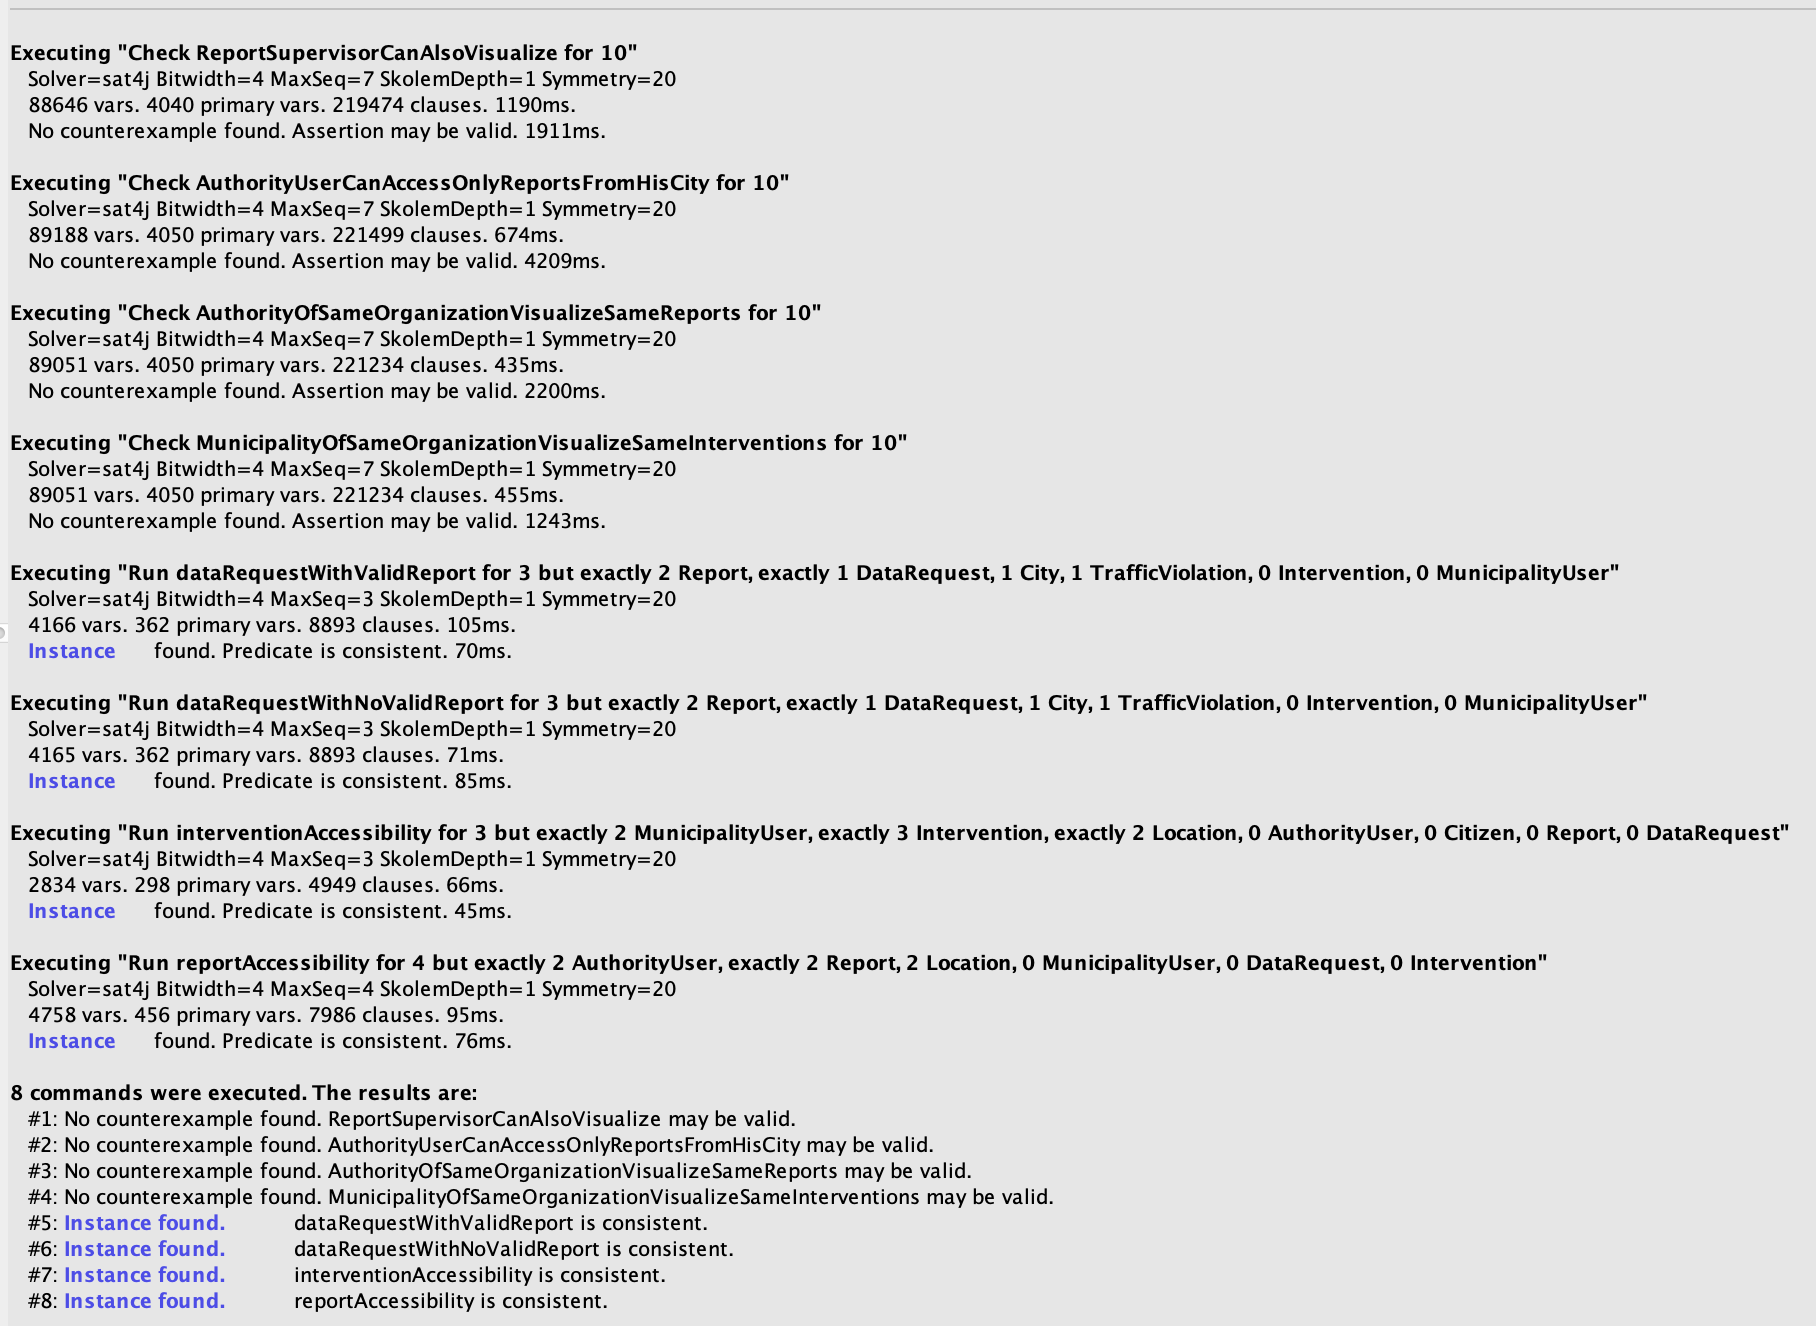
\includegraphics[width=\textwidth]{Alloy/execution}
	\caption{World execution details}
\end{figure}

In the following section we present some possible models of the world, in particular the continuous lines represents the most important relations, whereas the dotted lines represents the least important ones.
\begin{figure}[H]
	\centering
	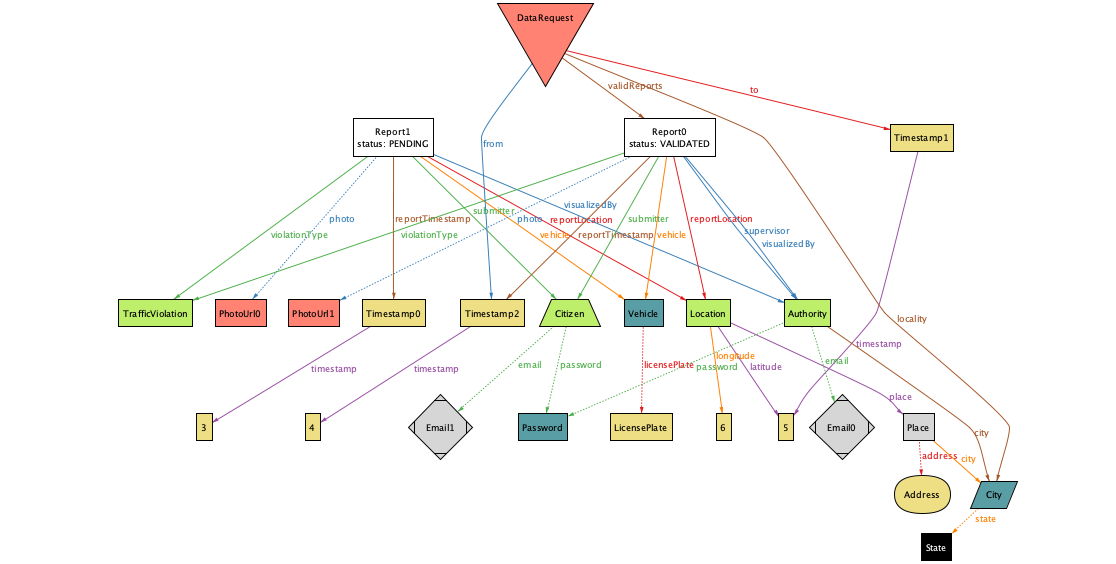
\includegraphics[width=\textwidth]{Alloy/dataRequestWithValidReport}
	\caption{World 1}
\end{figure}
In the first world, we can see that different users have different emails (used for registration and login) and there are two reports and one data request. The first report is in a pending status even though it is visualized by an authority that has in its jurisdiction the city where the violation occurred, and it is correctly among the reports associated to the data request. The second report is in a validated status, indeed there is an authority in that city who is its supervisor; also this report satisfies the time and spatial constraints of the data request so it is in its valid reports.
\begin{figure}[H]
	\centering
	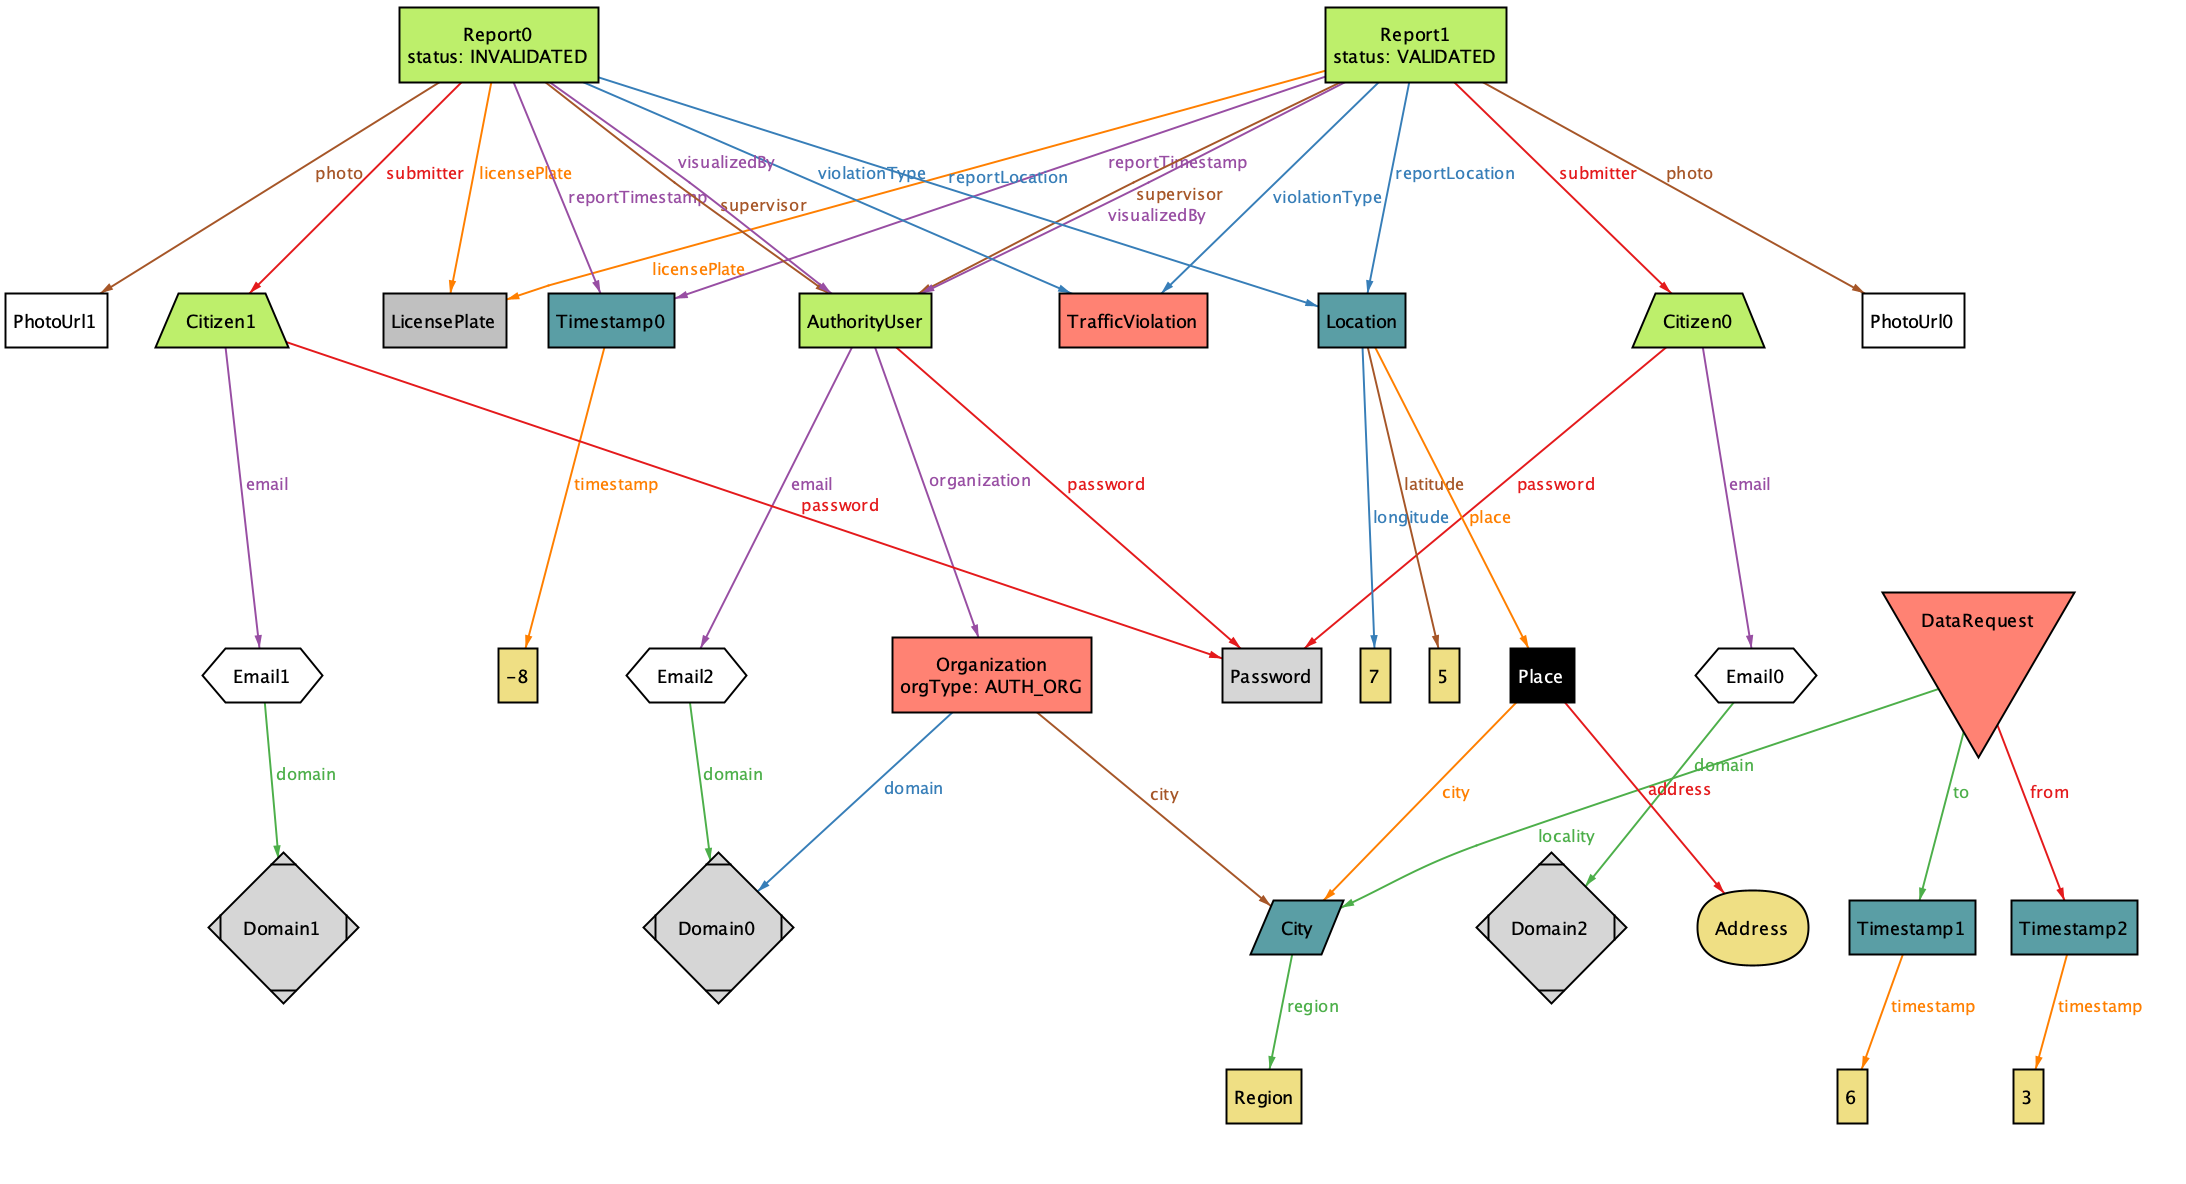
\includegraphics[width=\textwidth]{Alloy/dataRequestWithNoValidReport}
	\caption{World 2}
\end{figure}
In the second world, there is one validated request, one invalidated request and one data request. The two reports are about the same traffic violation (same vehicle, same location and same timestamp), but they are reported by different citizens with two different photos. It is interesting to see that the report of a same violation can be validated in one case and not in the other, most probably when a photo describes completely the violation situation and not respectively. In this case there are no reports in the data requests, because there are no reports satisfying its filter.
\begin{figure}[H]
	\centering
	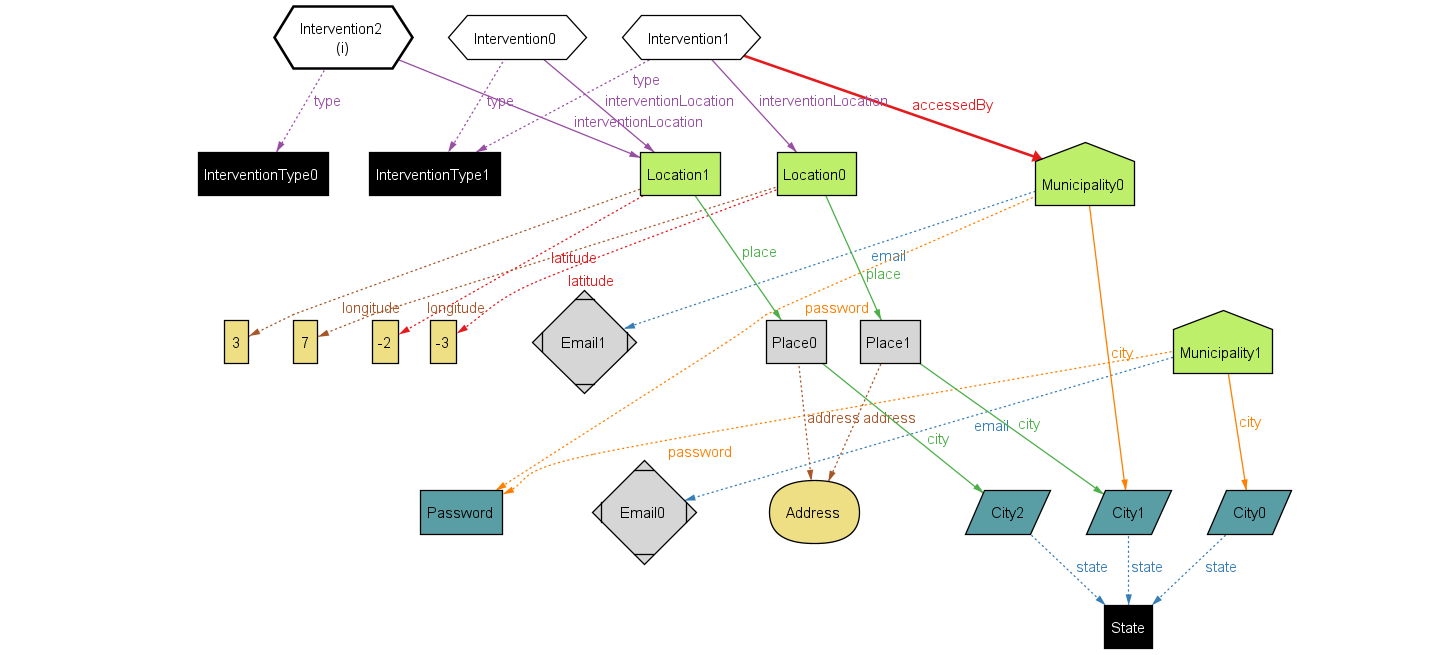
\includegraphics[width=\textwidth]{Alloy/interventionAccessibility}
	\caption{World 3}
\end{figure}

In the third world, we can check that an intervention can be seen only by municipality of the city in which the intervention is situated. As you can see, municipality1 can access intervention1 and intervention0 because their location is situated in the same city of it, same thing happens for intervention2 and municipality0. Some interventions can occur in the same location because different intervention type could be needed in that place.

\begin{figure}[H]
	\centering
	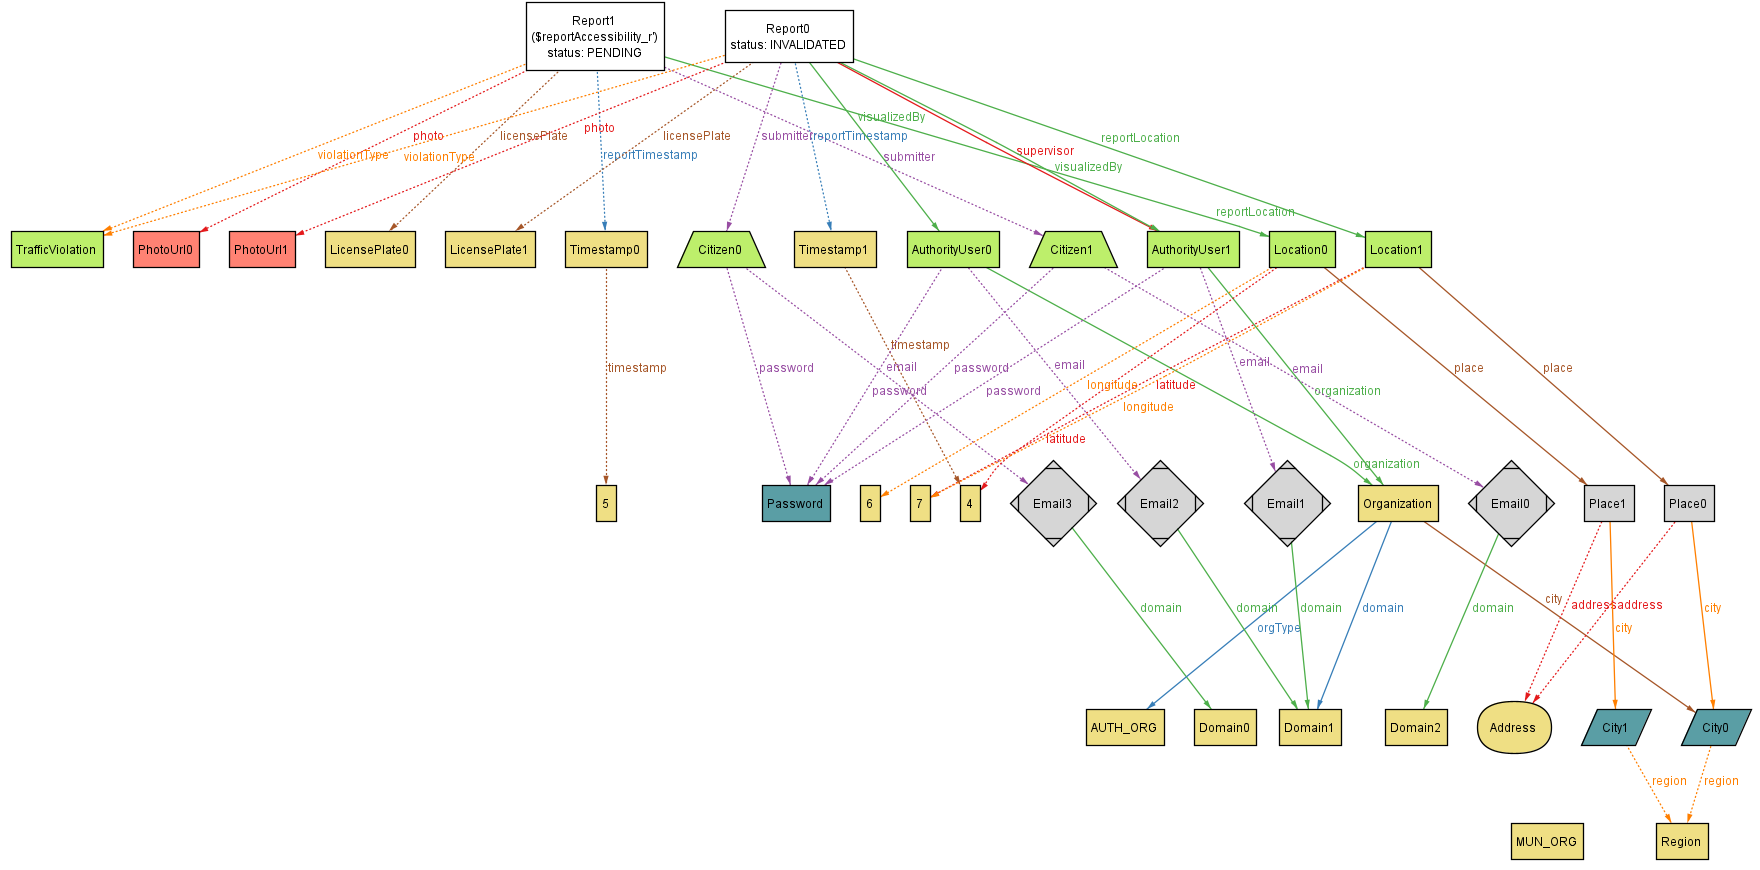
\includegraphics[width=\textwidth]{Alloy/reportAccessibility}
	\caption{World 4}
\end{figure}

In the fourth world, we can check that a report can be visualized only by authorities who have jurisdiction on that city. Another interesting relation is that report supervisor is of course an authority that can access it, also if a supervisor is present means that report is either validated or invalidated. If a report can't be accessed, clearly its status remain always pending because no authority can't change it.